\chapter{Numerical Methods for Open Quantum Systems}
\label{Chapter2}
As we have seen in the previous chapter, the study of an open quantum system requires the knowledge of its density matrix, solution of the Lindblad master equation~\cite{presk:quant_info}:
\begin{equation*}
    \dot{\rho} = \mathcal{L}[\rho],
\end{equation*}
where
\begin{equation}
\label{eqn:lindblad_eqn}
    \mathcal{L}[\rho] \equiv -i[H, \rho] +\sum_{a>0}\Bigl(L_a\rho L_a^{\dagger} - \frac{1}{2}L_a^{\dagger}L_a\rho - \frac{1}{2}\rho L_a^{\dagger}L_a\Bigl).
\end{equation}
In such a system the number of variables scales as the square of the dimension of the Hilbert space; for example, in a spin-$\frac{1}{2}$ system made up by $n$ elements, the size of the Hilbert space $\mathcal{H}$ is $2^n$ and we can say that the \emph{liouvillian dimension} equals to $2^{2n} \times 2^{2n}$. Clearly, a direct integration of the equation~\ref{eqn:lindblad_eqn} can be made only for systems with a very limited number of elements. One only needs to note the fact that for a brute-force integration of the ~\ref{eqn:lindblad_eqn} for a system consisting of $8$ sites, about $34$ GB of memory would be necessary\footnote{This calculation considers the fact that the liouvillian contains, in general, complex numbers, each of them valued with a single precision (32 bit).}.

So, it becomes undeniable that numerical techniques are required to solve these problems; in this section we will examine some of the most used at this time.

The numerical methods employed in open quantum system problems can be classified in  

\section{The Corner-Space Renormalization (CSR) Method}
\label{chapter2_csr}
The numerical methods based on renormalization group à la Wilson present a calculation problem due to the increase of the dimensions of the Hilbert space, while the blocks are merged; the fundamental aim of the corner-space renormalization method~\cite{PhysRevLett.115.080604} is to treat this problem.

The name of this method refers to the idea of selecting a \emph{corner} of the Hilbert space for a lattice system, using eigenvectors of the steady-state density matrix of smaller lattices.

Let us start considering two blocks of a quantum system consisting in a certain number $N$ of sites arranged to forming a 1D chain (the dimension of the system is not important at this stage, but in this thesis it will be one of the central topics). The CSR approach is a recursive process that begins with the calculation of the steady-state density matrix of a small block (the first \emph{block} will be a single site, in the second iteration it will be a small lattice constituted of the two blocks emerged in the previous iteration, and so on); this calculation can be done studying the spectrum of the eigenvalue of the Liouvillian and taking the zero value, considered that:
\begin{equation}
    \frac{d\rho}{dt} = \mathcal{L} \rho.
\end{equation}
We now consider two spatially adjacent sites; the site A and the site B. We now call $\rho^{(A)}$ the steady-state density matrix of the first site and $\rho^{(B)}$ of the latter. In order to spatially merge these two sites, let us write $\rho^{(A)}$ and $\rho^{(B)}$ in terms of an orthonormal basis; if there is no degeneracy among eigevalues of $\rho^{(A)}$ and $\rho^{(B)}$, we can use the orthonormal basis formed by their eigenvectors. Instead, if there is degeneration, a Gram-Schmidt orthonormalization process can be used to obtain an orthonormal basis starting from the ensemble of eigenvectors.

In this way, we will have:
\begin{equation}
    \rho^{(A)} = \sum_r p_r^{(A)}\ket{\phi_r^{(A)}}\bra{\phi_r^{(A)}},
\end{equation}
\begin{equation}
    \rho^{(B)} = \sum_{r'} p_{r'}^{(B)}\ket{\phi_{r'}^{(B)}}\bra{\phi_{r'}^{(B)}}.
\end{equation}
The steady-state density matrix of the \emph{merged block} constituted of the block A and the block B will be the following:
\begin{align}
\label{rhoAUB}
    \rho^{(AUB)} &= \rho^{(A)} \otimes \rho^{(B)} = \\
    \label{rhoAUB_explicit}
    &= \sum_{r} \sum_{r'} p_r^{(A)}p_{r'}^{(B)}\ket{\phi_r^{(A)}}\ket{\phi_{r'}^{(B)}} \otimes \bra{\phi_{r'}^{(B)}}\bra{\phi_{r}^{(A)}}
\end{align}
At this point, the CSR method suggests to delineate the \emph{corner-space}; for this purpose, we consider the $M$ most probable product states coming from~\ref{rhoAUB} of the form $\ket{\phi_{r}^{(A)}}\ket{\phi_{r'}^{(B)}}$, i.e. we rank the~\ref{rhoAUB_explicit} according to the joint probability $p_r^{(A)}p_{r'}^{(B)}$. The $M$ states form an orthonormal basis that generates a subspace
\begin{equation}
\label{basis_corner}
    \Bigl\{\ket{\phi_{r_1}^{(A)}}\ket{\phi_{r_1'}^{(B)}}, \ket{\phi_{r_2}^{(A)}}\ket{\phi_{r_2'}^{(B)}}, \dots, \ket{\phi_{r_M}^{(A)}}\ket{\phi_{r_M'}^{(B)}} \Bigl\},
\end{equation}
called \emph{corner-space}, with
\begin{equation*}
    p_r_1^{(A)}p_{r_1'}^{(B)} \geq p_r_2^{(A)}p_{r_2'}^{(B)} \geq \dots \geq p_r_M^{(A)}p_{r_M'}^{(B)}.
\end{equation*}
So, now it becomes necessary doing a change of basis to the new block $A \cup B$, that is:
\begin{equation}
    H' = \tilde{O} H_{A\cup B} \tilde{O}^\dagger,
\end{equation}
where $\tilde{O}$ is a pseudo-orthogonal\footnote{The matrix $\tilde{O}$ is called pseudo-orthogonal because it is not a square matrix.} $M\times N$ matrix, where $N$ is the dimension of $H_{A\cup B}$; $\tilde{O}$ is formed by the $M$ eigenvectors of $\rho_{A\cup B}$ living in the corner-space. This density matrix can now be used to calculate the expectation values of observable.

The more $M$ is large, the more the results are exact, because the basis~\ref{basis_corner} spans a larger part of the Hilbert space. Therefore, at this point the value of $M$ should be increased until the convergence is reached.

In the work of~\cite{PhysRevLett.115.080604}, as in the present thesis, has been proved that convergence can be achieved with a number of states $M$ much smaller than the dimension of the Hilbert space.

%The resulting dimension of the space in which, from now on - re-iterating the procedure - the system will be studied, is made smaller.

\bigskip
In short, the algorithm is structured in the following stages, as sketched in the FIG:
\begin{description}
    \item[calculation] of the steady-state density matrix of a single block of the system;
    \item[merger] of two predetermined blocks;
    \item[expression] of the density matrix of the merged block in an orthonormal basis;
    \item[selection] of the M most probable states as a basis for the so-called \emph{corner-space};
    \item[increase] of the dimension M of the corner-space until the convergence of the observable is achieved.
\end{description}

A detailed description of the implementation of the algorithm can be seen in~\ref{AppendixA}.


\section{The Quantum Trajectories (QT) Method}
A completely different approach is reached in the \emph{quantum trajectories method}, in which pure states are the subjects of the study, instead of density matrices. This means that a vector of length $N$ (where $N$ is the dimension of the Hilbert space) is stored, rather than a matrix of dimensions $NxN$.

The idea of this method can be summarised in the following way.

First of all, given the~\ref{eqn:lindblad_eqn}, let us note that the \textbf{first three terms} of this equation can be regarded as the evolution performed by an effective non-Hermitian Hamiltonian, that is~\cite{PhysRevA.69.062317}:
\[
H_{eff} = H_s + \rm{i}K,
\]
with
\[
K = -\frac{\hbar}{2}\sum_\mu L_{\mu}^{\dagger}L_{\mu}.
\]
In fact, we see that:
\[
    -\frac{\rm{i}}{\hbar}[H_{eff}, \rho] = -\frac{\rm{i}}{\hbar}[H_s, \rho] - \frac{1}{2}\sum_\mu \{L_{\mu}^{\dagger}L_{\mu}, \rho\}.
\]

The \textbf{last term} of the~\ref{eqn:lindblad_eqn}, is the one responsible for the so-called \emph{quantum jumps}; for this reason, the representation under which we have written the~\ref{eqn:lindblad_eqn} is called \emph{quantum jump picture}~\cite{PhysRevA.69.062317}. 

At an initial time $t_0$, the density matrix of the system is in a pure state
\[
\rho(t_0) = \ket{\phi(t_0)}\bra{\phi(t_0)};
\]
after a time $dt$, it evolves to the following statistical mixture:
\begin{equation}
    \rho(t_0 + dt) = \Bigl(1-\sum_\mu dp_\mu \Bigl)\ket{\phi_0}\bra{\phi_0} + \sum_\mu dp_\mu \ket{\phi_\mu}\bra{\phi_\mu},
\end{equation}
where
\begin{equation}
    dp_\mu = \bra{\phi(t_0)}L_{\mu}^{\dagger}L_{\mu}\ket{\phi(t_0)}dt
\end{equation}
is the probability that a jump occurs; in this case, the system evolves in the state
\begin{equation}
\label{eqn:phi_mu}
    \ket{\phi_\mu} = \frac{L_\mu}{\abs{L_\mu\ket{\phi(t_0)}}}\ket{\phi(t_0)}.
\end{equation}
Otherwise, if no jump happens, the system evolves according to the effective Hamiltonian $H_{eff}$ in the following way:
\begin{equation}
    \ket{\phi_0} = \frac{(1-\textrm{i}H_{eff}dt/\hbar)}{\sqrt{1-\sum_\mu dp_\mu}}\ket{\phi(t_0)}.
\end{equation}

In order to decide if the jump occurs or not, a Monte Carlo method will be integrated in this picture. Namely, an uniform distribution in the unit interval $[0,1]$ is taken under consideration; for every experiment, a pseudo-random number $\epsilon$ is chosen from this uniform distribution, i.e. a coin is tossed: depending on the result of the throw, the possible situations are the following:
\begin{itemize}
    \item if $\epsilon < \sum_\mu dp_\mu$, the system jumps to one of the states $\ket{\phi_\mu}$, defined in~\ref{eqn:phi_mu}. In particular:
    \begin{itemize}
        \item if $0 \leq \epsilon \leq dp_1$, the system jumps to $\ket{\phi_1}$;
        \item if $dp_1 < \epsilon \leq dp_2$, the system jumps to $\ket{\phi_2}$;
        \item and so on;
    \end{itemize}
    \item if $\epsilon > \sum_\mu dp_\mu$, the system evolves to the state $\ket{\phi_0}$.
\end{itemize}

This process has to be repeated as many times as $n = \frac{T}{dt}$, where $T$ is the whole elapsed time during the evolution. Let us note that $dt$ must be taken much smaller than the evolution time of the system.

Every \emph{experiment}, i.e. every throw of the coin, gives a different \emph{quantum trajectory}, which can be used to calculate the mean value of an observable $A$ at a certain time $t$, in this way:
\begin{equation}
    \langle A(t)\rangle = \bra{\phi_i(t)}A\ket{\phi_i(t)}.
\end{equation}
Since this is a result of a Monte Carlo process, a good idea to obtain a reasonable outcome is to repeat the \emph{experiment} a number $N$ of times and to take the mean value of the results:
\begin{equation}
    \langle A(t)\rangle = \lim_{N\to\infty} \frac{1}{N}\sum_{i=1}^{N}\bra{\phi_i(t)}A\ket{\phi_i(t)}.
\end{equation}


\section{The Matrix Product Density Operators (MPDO) Method}
The last numerical method analyzed in this overview, is the \emph{matrix product density operators method} (MPDOM).
This method is rooted in one of the first and most efficient numerical methods: the \emph{density matrix renormalization group} (DMRG)~\cite{s_white:dmrg}. The reason why the DMRG is a powerful method is because the many-body states of some 1D problems can be described in terms of the so-called \emph{matrix product states} (MPS)~\cite{PhysRevLett.93.207204, PhysRevLett:from_dmrg_to_mps}:
\begin{equation}
    \ket{\psi_{MPS}} = \sum_{i_1, ..., i_N = 1}^{d} \Tr(A^{[1]i_N}...A^{[N]i_N}) \ket{i_1,...,i_N},
\end{equation}
where the $A$'s are matrices with dimensions $\chi$ and $d$ is the dimension of the Hilbert space of every sub-system $i_k$. The total number of parameters turns out to be $N \times d \times \chi^2$, i.e. linear in $N$.

The matrix product \emph{density operators} (MPDO) extend the MPS from pure to mixed states, following the idea explained, for example, in~\cite{PhysRevLett.93.207204}. 
\begin{equation}
\label{eqn:mpdo}
    \rho = \sum_{i_1, \dots ,i_N = 1}^{d} \sum_{j_1, \dots ,j_N = 1}^{d} \Tr\Bigl(A^{[1]i_1,j_1} \dots A^{[N]i_N,j_N}\Bigl) \ket{i_1, \dots ,i_N}\bra{j_1, \dots ,j_N},
\end{equation}
where $A^{[k]i_k,j_k}$ are $\chi^2 \times \chi^2$ matrices that can be written in this way:
\begin{equation}
    A^{[k] i,j} = \sum_{a = 1}^{d_k} B_k^{i,a} \otimes (B_k^{j,a})^*.
\end{equation}

Another way of considering the expression~\ref{eqn:mpdo} is the graphical notation to represent a tensor $A^{[k] i,j}$ sketched in figure~\ref{fig:tensor_network}. Here, every tensor is represented by a square with 4 links: two for the bonds with the neighbours, two are the physical indices instead (the "bras" and "kets"). 

\begin{figure}[H]
    \centering
    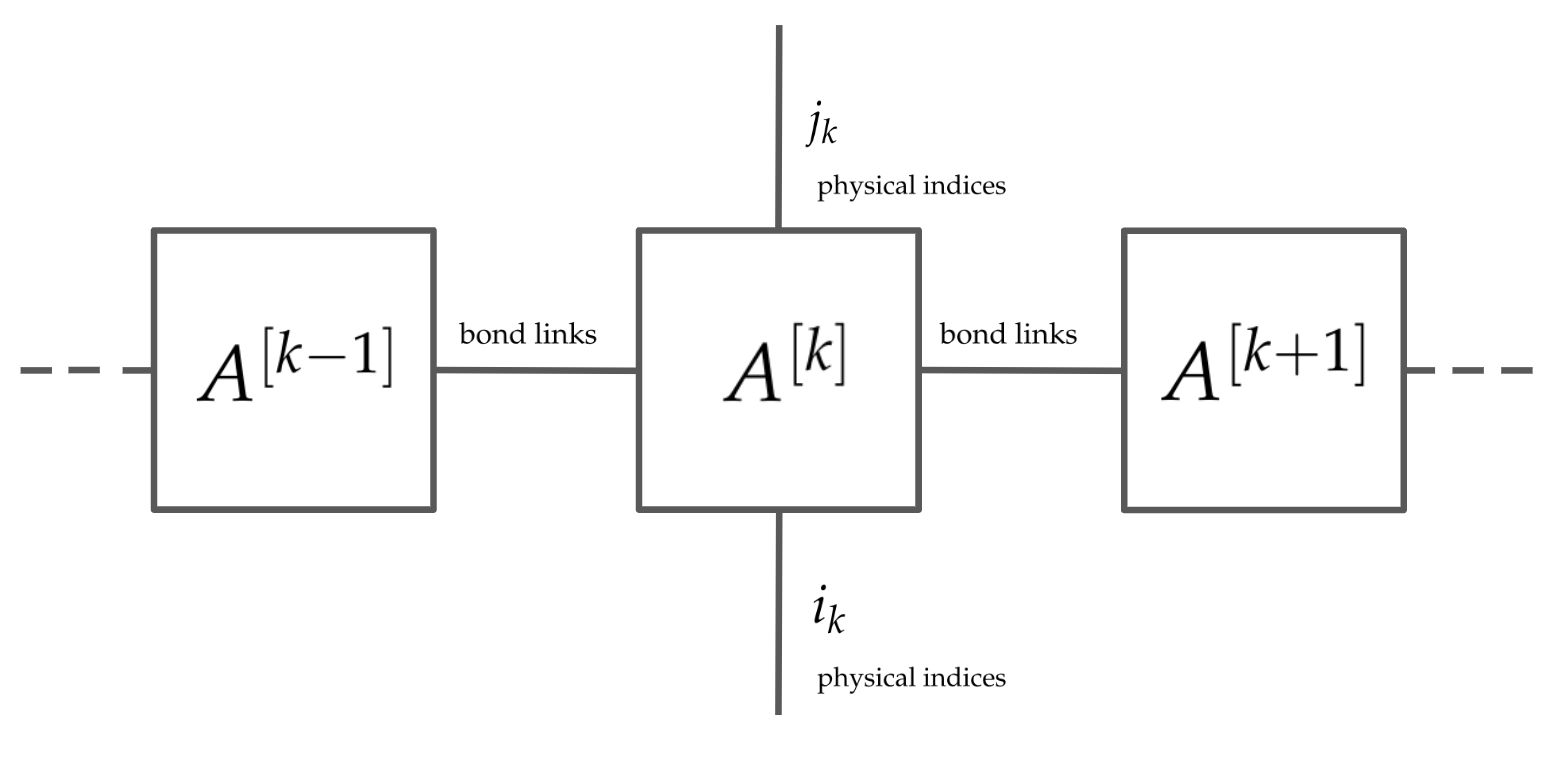
\includegraphics[scale=0.30]{Figures/tensor_network.png}
    \caption{Graphical notation of tensors in a 1D system.}
    \label{fig:tensor_network}
\end{figure}




%\noindent\rule[0.5ex]{\linewidth}{1pt}
%\noindent\rule[0.5ex]{\linewidth}{1pt}

%One can express a MPDO in terms of a pure state MPS using the \emph{purification}~\cite{nielsen_chuang} technique. The essential idea is to consider an auxiliary system with a Hilbert space of dimension $d_k$ and, after choosing an orthonormal basis $\ket{i_k, a_k}$, to write the corresponding MPS state as
%\begin{equation}
%    \ket{\psi} = \sum_{i_1,\dots,i_N} \sum_{a_1, \dots, a_N} Tr\Bigl(\prod_{k=1}^N B_k^{i_k, a_k}\Bigl) \ket{i_1a_1, \dots, i_Na_N}.
%\end{equation}
%and eventually the MPDO $\rho$ is obtained tracing over the indices referred to the auxiliary system $a_k$:
%\begin{equation}
%    \rho = Tr_a(\ket{\psi}\bra{\psi});
%\end{equation}
%this density matrix can be used to compute the expectation values of observables.